\section{Entorno de Desarrollo Local}

Para garantizar la reproducibilidad del proyecto, en esta sección se descibirá el entrono de desarrollo en el que se ha realizado y el acceso al repositorio con el código fuente.

\subsection{Tecnologías y Versiones}

El proyecto se ha desarrollado en un entorno \textbf{Windows 10}, aunque esto no influye en la compatibilidad, ya que todas las tecnologías utilizadas son multiplataforma, lo cual permite realizar el desarrollo en cualquier sistema operativo sin restricciones. En la tabla \ref{tab:dependencias_versiones} se presentan las tecnologías principales empleadas en el proyecto junto con sus versiones correspondientes.

\begin{table}[htbp]
    \centering
    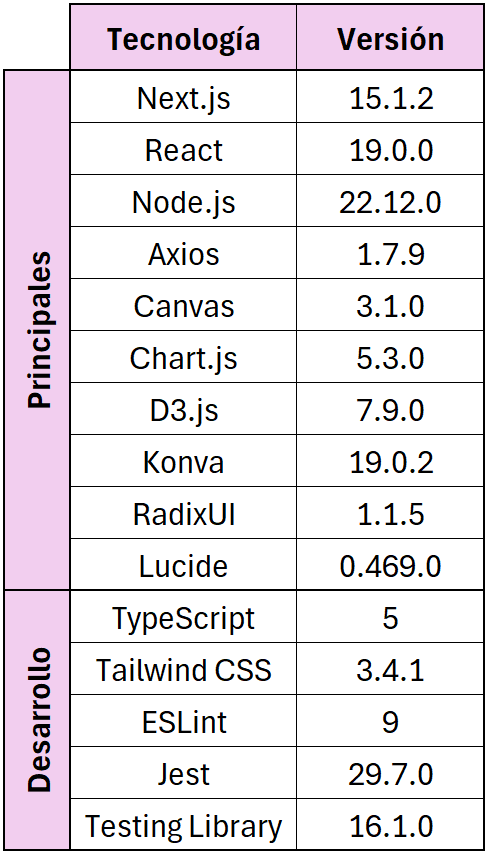
\includegraphics[width=0.37\textwidth]{figures/dependencias_versiones.png}
    \captionsetup{skip=5pt}
    \caption{Dependencias usadas en el desarrollo, junto con sus versiones.}
    \label{tab:dependencias_versiones}
\end{table}

Cabe destacar que el gestor de paquetes utilizado en el proyecto ha sido \textbf{\texttt{pnpm} (\textit{Performant Node Package Manager})}, en lugar de \texttt{npm} (\textit{Node Package Manager}) o \texttt{yarn} (\textit{Yet Another Resource Negotiator}). La elección de \texttt{pnpm} se debe a sus mejoras en la gestión de dependencias y optimización del uso del espacio de almacenamiento. A diferencia de \texttt{npm}, \texttt{pnpm} utiliza un sistema de enlaces en lugar de duplicar archivos en cada proyecto, lo que reduce significativamente el consumo de espacio. Además, \texttt{pnpm} es completamente compatible con los paquetes del registro de \texttt{npm}, lo que garantiza su interoperabilidad con la mayoría de los ecosistemas de desarrollo basados en \textit{Node.js}.

\subsection{Instalación y Configuración del Proyecto}

El proyecto se encuentra alojado en un repositorio de \textit{GitHub}\footnote{Repositorio del proyecto: \href{https://github.com/jonortega/tfg-app-spotify}{https://github.com/jonortega/tfg-app-spotify}} para evitar pérdidas y tener disponibilidad completa al código. Para ejecutarlo localmente, además de haber instalado \textit{Node.js}, hay que clonar el respositorio, acceder a la carpeta y ejecutar los comandos de instalación y ejecución. A continuación, se muestran los comandos necesarios para realizar estos pasos:

\begin{ifalgorithm}[H]
    \begin{lstlisting}[language=bash]
    # Clonar el repositorio
    git clone https://github.com/jonortega/tfg-app-spotify.git
    
    # Acceder al directorio del proyecto
    cd tfg-app-spotify
    
    # Instalar dependencias
    pnpm install
    
    # Ejecutar el servidor de desarrollo
    pnpm run dev
    \end{lstlisting}
    \caption{Comandos de instalación y ejecución inicial del proyecto.}
    \label{alg:instalacion_proyecto}
\end{ifalgorithm}

Tras estos pasos, la página web estará accesible en \texttt{localhost:3000}. Es encesario agregar un fichero de variables de entorno \texttt{.env.local}, ya que, por seguridad, no se registra en el sistema de control de versiones. El contenido de dicho fichero se muestra en el \hyperref[ch:anexoC]{Anexo C} (algoritmo \ref{alg:variables_entorno}).

Dos de las variables de entorno necesarias para poder tratar con la API de \textit{Spotify}, son el \textbf{Client ID} y el \textbf{Client Secret}. Estos dos valores se obtienen al realizar el registro de la aplicación en la plataforma de desarrollo de \textit{Spotify}. En la siguiente sección, se explicará cómo realizar este registro y dónde obtener dichas variables.

\newpage

\section{Registro de la Aplicación en Spotify}

Para poder obtener datos de la Web API de \textit{Spotify}, es necesario registra la aplicación en su plataforma de desarrollo\footnote{Spotify for Developers: \href{https://developer.spotify.com/}{https://developer.spotify.com/}}. Tras inciar con una cuenta, se nos presentará un panel donde podremos crear una nueva app. \textit{Spotify} pedirá algunos datos (figura \ref{fig:create_app}), que tendremos que rellenar. Los campos como \textit{Redirect URIs} pueden ser modificados posteriormente, ya que tendremos que actualizarlo con el dominio indicado tras el despliegue de la aplicación.

\begin{figure}[H]
    \centering
    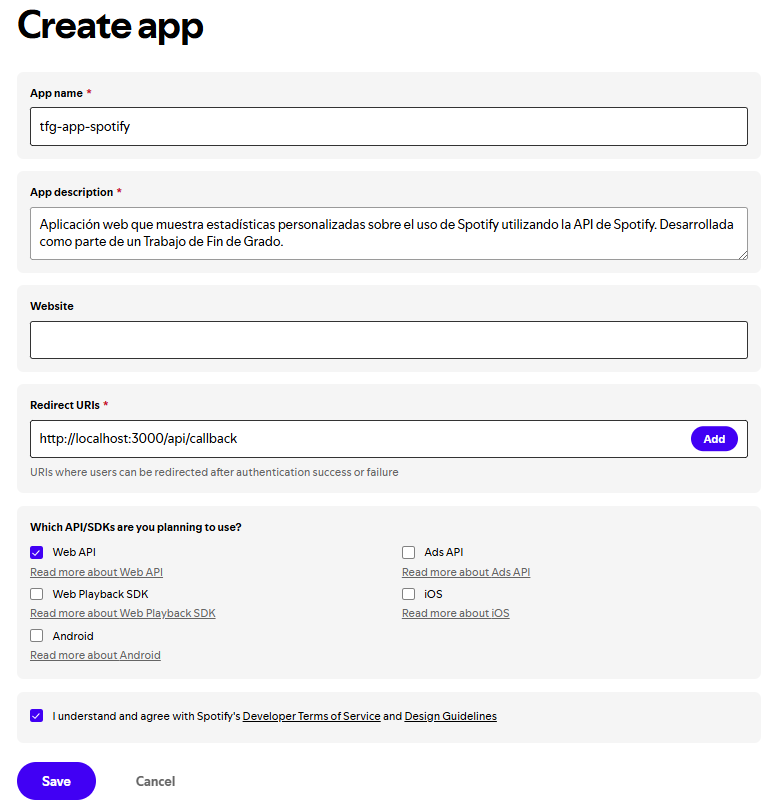
\includegraphics[width=0.65\textwidth]{figures/registro_spotify/create_app.png}
    \caption{Panel de creación de app en la plataforma de \textit{Spotify}.}
    \label{fig:create_app}
\end{figure}

Al aceptar los términos y crear la app, tendremos acceso al \textit{Client ID} y \textit{Client Secret}. Estos se encuentran en los ajustes (\textit{settings}) y tendremos que expandir el panel para poder ver los dos valores (figura \ref{fig:client_id_secret}).

\begin{figure}[H]
    \centering
    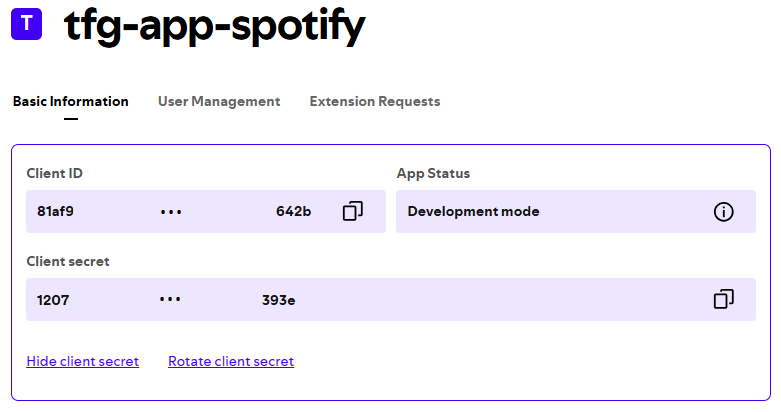
\includegraphics[width=0.65\textwidth]{figures/registro_spotify/client_id_secret.png}
    \caption{Panel de ajustes con el \textit{Client ID} y el \textit{Client Secret}.}
    \label{fig:client_id_secret}
\end{figure}

En el caso en el que el \textit{Client Secret} haya sido comprometido, es posible generar uno nuevo, anulando el anterior y evitando tener que desechar la aplicación registrada. También se muestra un campo llamado \textit{App Status} con el valor \textbf{Development Mode}. Esto significa que la aplicación registrada está en ``desarrollo'', por lo que existen las siguientes restricciones:

\begin{itemize}
    \item Un máximo de 25 usuarios (cuentas verificadas de \textit{Spotify}) pueden usar la aplicación.
    \item Cada usuario tiene que estar registrado en una lista de permitidos (\textit{allowlist}) de la plataforma.
\end{itemize}

Es posible eliminar estas restricciones, enviando una solicitud a \textit{Spotify} para cambiar el estado de \textit{Development Mode} a \textbf{Extended Quota Mode}. En el caso de que sea aceptada, se elimina cualquier restricción sobre el número de usuarios permitidos y no será necesario registrarlos anteriormente, además de ampliar el umbral de la tasa de peticiones (\textit{rate limit}). En este trabajo \textbf{no se va a realizar dicha solicitud}, por lo que tendremos que acogernos a las limitaciones impuestas en el modo de desarrollo. Esto requiere que se registren las cuentas de usuarios que vayan a probar la aplicación en la pestaña de gestión de usuarios (figura \ref{fig:user_management}).

\begin{figure}[H]
    \centering
    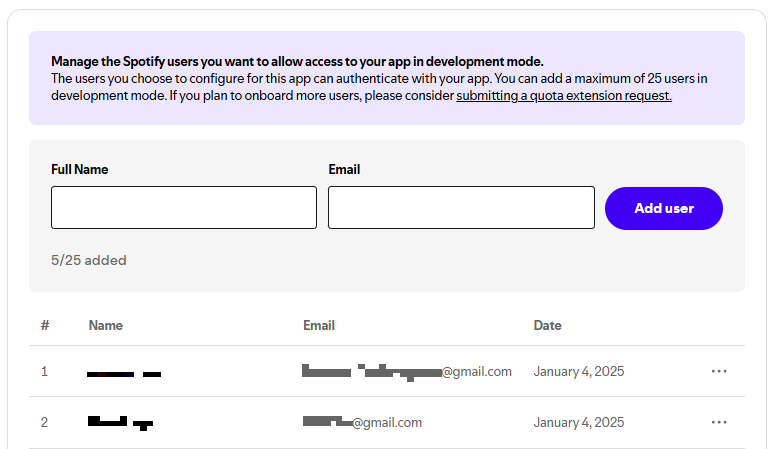
\includegraphics[width=0.75\textwidth]{figures/registro_spotify/user_management.png}
    \caption{Panel de gestión de usuarios que tienen acceso a la aplicación.}
    \label{fig:user_management}
\end{figure}

Con estos pasos, se habrá realizado correctamente el registro de la aplicación y obtención del \textit{Client ID/Secret}, imprescindibles para la comunicación con la API de \textit{Spotify}. En la plataforma de desarrollo, además, tenemos accesible un panel para poder monitorear la actividad de la aplicación (\hyperref[ch:anexoC]{Anexo C}, figura \ref{fig:dashboard_spotify}).

\section{Ciclo de Desarrollo}

El ciclo de desarrollo del proyecto ha seguido un enfoque híbrido entre los modelos \textbf{incremental} e \textbf{iterativo}. En concreto, se ha construido en tres incrementos, realizados en diferentes puntos del proyecto. En cada uno, se han añadido más funcionalidades (incremental) y refinando las ya existentes (iterativo). A continuación se describe cada incremento con más detalle.

\subsection*{Incremento I: Prototipado Rápido}

Durante la fase inical de adquisición de competencias, se desarrolló un prototipo rápido para validar la viabilidad técnica del proyecto. No se buscaba crear la base desde donde seguir trabajando una vez inicase el desarrollo formal; si no que, utilizando herramientas más simples, se quería obtener una idea preliminar de cómo se podrían implementar las funcionalidades principales. No se utilizaron las tecnologías finales del desarrollo, por lo que gran parte del código implementado no fue reutilizado.

En este prototipo se implementaron las siguientes funcionalidades, en diferentes grados de completado:
\setlength{\itemsep}{0pt}
\begin{itemize}
    \item Inicio de sesión de un usuario y obtención de los tokens.
    \item Renovación del \texttt{access\_token} mediante el \texttt{refresh\_token}.
    \item Obtener los \textit{top items} del usuario.
    \item Obtener las canciones favoritas del usuario.
    \item Obtener los \textit{track features} (\textbf{no implementado en el producto final}).
    \item Prototipos de las estadísticas:
          \begin{itemize}
              \item \textit{Hall Of fame}
              \item \textit{Huella Del Día}
              \item \textit{La Bitácora}
          \end{itemize}
\end{itemize}

\subsection*{Incremento II: Producto Mínimo Viable (PMV)}

Una vez terminada la planificación del proyecto, se dio comienzo a una primera implementación del sistema, desarrollando una base de código que formaría parte del producto final. En esta fase, se utilizaron todas las tecnologías finales seleccionadas para el desarrollo, incluyendo \textit{Next.js}, \textit{React}, TypeScript y \textit{Tailwind CSS}.

Durante este incremento, se completaron las siguientes partes fundamentales del sistema:

\setlength{\itemsep}{0pt}
\begin{itemize}
    \item Estructura completa de páginas de la aplicación web.
    \item Implementación de los endpoints mediante \textit{Route Handlers}.
    \item Inicio de sesión y cierre de sesión seguros.
    \item Gestión segura de los tokens.
    \item Implementación de las estadísticas básicas \textit{Top Tracks}, \textit{Top Artists}, \textit{Top Genres} y \textit{Recently Played}.
    \item Desarrollo inicial de las seis estadísticas avanzadas finales en un estado funcional básico.
\end{itemize}

Si bien estas estadísticas se implementaron de manera inicial y sin refinamientos, su propósito principal fue definir la interacción entre el frontend y el backend, establecer los tipos de datos y endpoints exactos requeridos, y detectar posibles problemas en la presentación de la información. Asimismo, esta fase permitió identificar la necesidad de herramientas adicionales, como bibliotecas de gráficos, en caso de que las opciones disponibles no fueran suficientes.

En términos generales, este incremento sirvió para caracterizar con mayor precisión el alcance del proyecto y definir con claridad los aspectos que deberían considerarse en las siguientes etapas de análisis y diseño. A diferencia del prototipo inicial, gran parte del código desarrollado en esta iteración se integró directamente en la versión final del sistema.

\subsection*{Incremento III: Producto Final}

Finalmente, en el último incremento se completaron todas las funcionalidades secundarias pendientes, junto con una serie de optimizaciones de rendimiento, ajustes en las estadísticas avanzadas y mejoras en la interfaz y experiencia de usuario. Esta fase marcó la consolidación del sistema y la preparación del código para su despliegue.

Las principales funcionalidades implementadas y correcciones realizadas fueron:

\setlength{\itemsep}{0pt}
\begin{itemize}
    \item Posibilidad de cambiar el rango temporal en los módulos \textit{Top Tracks}, \textit{Top Artists} y \textit{Top Genres}.
    \item Implementación de la funcionalidad para crear playlists en \textit{Hall Of Fame}.
    \item Desarrollo de la estadística \textit{Tus Décadas} utilizando la librería \textit{Konva} para una mayor optimización.
    \item Mejora en la presentación y rendimiento de la estadística \textit{Índice de Interferencia} con \textit{D3.js}.
    \item Corrección en la estructura de datos enviada desde el backend a la estadística \textit{La Bitácora}.
    \item Implementación de la ventana informativa sobre la \textit{Política de Privacidad}.
    \item Reemplazo de la implementación manual de la ventana modal de las estadísticas por la librería \textit{Radix UI}.
    \item Creación de componentes de carga (\textit{loading components}).
    \item Gestión de errores encontrados al probar con diferentes cuentas de usuario.
    \item Desarrollo de una pantalla de carga específica para las estadísticas avanzadas.
    \item Refactorización del código para crear funciones reutilizables, como en la obtención de datos (\textit{fetch}), facilitando la gestión de los componentes.
    \item Preparación del código para su despliegue en \textit{Vercel}, especialmente la gestión de variables de entorno.
\end{itemize}

Este último incremento permitió completar todas las funcionalidades planeadas y refinar el sistema en su conjunto. Además de las mejoras implementadas, se documentaron posibles optimizaciones futuras, aunque, dentro del alcance definido para el proyecto, la aplicación alcanzó un estado final funcional y estable.

Cabe destacar que las listas de funcionalidades y mejoras descritas en cada incremento no son exhaustivas, sino que recogen las implementaciones y cambios más relevantes realizados durante el desarrollo. A lo largo del proceso, se llevaron a cabo numerosas correcciones, ajustes e implementaciones adicionales que no se han detallado en su totalidad. No obstante, estas listas permiten ofrecer una visión general de los aspectos más significativos de cada incremento en el desarrollo del proyecto.

\section{Gestión Segura de los Tokens}

Como se ha descrito anteriormente en la sección de \nameref{sec:diseno_seguridad}, se han tomado ciertas medidas a la hora de gestionar los tokens que permiten la interacción con la API de \textit{Spotify}. En primer lugar, el \textit{Client ID} y \textit{Client Secret} se alamacenan en el servidor, en respectivas variables de entorno, y solo se acceden desde el objeto \texttt{process.env}. Estos tokens nunca son enviados al cliente y se usan en casos concretos, como en el inicio de sesión de un nuevo usuario o la renovación del \texttt{access\_token}.

Por otro lado, la gestión del propio \texttt{access\_token} requiere más atención. Se evaluaron varias opciones, pero finalmente se decidió en hacer uso de las \textbf{cookies}. Esto se debe a que, de esta manera, no era necesario implementar un sistema de almacenamiento en el servidor (manual o mediante herramientas como \textit{Redis}) para guardar los \texttt{access\_token} de los diferentes usuarios y asociarlos a un identificador único. El propio \texttt{access\_token} hace de identificador de cada usuario, por lo que el servidor solo tiene que hacer uso del token recibido mediante las cookies agregadas en la petición.

No obstante, es importante utilizar los sistemas de seguridad que las propias cookies ofrecen, para limitar cualquier tipo de uso malintencionado del token. Existen ciertas opciones (\textit{flags}) de configuración que se han establecido:

\setlength{\itemsep}{0pt}
\begin{itemize}
    \item \textbf{httpOnly}: \textbf{Impide que el token sea accesible mediante JavaScript en el navegador}, protegiéndolo contra ataques de tipo \textit{Cross-Site Scripting} (XSS).
    \item \textbf{secure}: Se asegura de que las cookies \textbf{solo sean enviadas a través de conexiones HTTPS}, protegiéndolas contra ataques de interceptación de tráfico (\textit{Man-in-the-Middle}, MITM). Esta opción solo se habilita cuando la aplicación se ejecuta en un entorno de producción.
    \item \textbf{maxAge}: Define el tiempo de \textbf{expiración de las cookies}. El \texttt{access\_token} tiene una validez de una hora, mientras que el \texttt{refresh\_token} se mantiene activo durante 24 horas, permitiendo la renovación del token de acceso sin necesidad de solicitar credenciales nuevamente.
\end{itemize}

Estableciendo de esta manera el \texttt{access\_token} y el \texttt{refresh\_token} en las cookies y enviándolas en la respuesta al cliente, se mantiene la posibilidad de que cada usuario envíe su propio token como identificador, pero manteniendo la seguridad frente a ataques comunes. También se debe mencionar que, por el hecho de haber habilitado el \textit{flag} \texttt{httpOnly}, \textbf{ningún componente de cliente puede realizar peticiones directamente desde el neavegador}. Todas las peticiones de datos a la API de \textit{Spotify} deben de ser realizadas a tráves del backend seguro.

\subsection*{Implicaciones de la Decisión del uso de las Cookies}

El uso de las cookies como forma de almacenamiento del identificador también requiere el conocimiento del alcance efectivo de este sistema, que permite identificar posibles limitaciones que este método impone. Las cookies son compartidas entre todas las pestañas y ventanas del mismo navegador mientras se mantengan dentro del mismo dominio, lo que permite que la autenticación y la sesión del usuario se mantengan consistentes en diferentes contextos de navegación. Estas no se comparten entre distintos navegadores, ya que cada uno gestiona su propio almacenamiento de cookies.

Sin embargo, este sistema es \textbf{vulnerable si un atacante tiene acceso físico a la máquina} del usuario con la sesión abierta. A través del panel de desarrollador del navegador, el atacante podría visualizar directamente los valores de los tokens almacenados en las cookies. Aunque este método de almacenamiento impide el acceso mediante sistemas automatizados, un atacante con acceso manual al dispositivo podría extraer y utilizar estos valores.

Una posible medida de mitigación sería cifrar los tokens antes de almacenarlos en las cookies. No obstante, \textbf{se ha decidido no implementar esta solución} debido a varias razones: en primer lugar, por las limitaciones de alcance del proyecto; en segundo lugar, por la carga computacional adicional que supondría para el servidor el proceso de cifrado y descifrado en cada solicitud del usuario; y, finalmente, porque se considera que la probabilidad de que un atacante tenga acceso físico a una sesión abierta del usuario es extremadamente baja, lo que no justifica la implementación de este mecanismo en un sistema de estas características.

% \section{Implementación del Fronted}

% \subsection{React Hooks}

% Uno de los conceptos más importantes de \textit{React} son los \textbf{Hooks}. Estos permiten gestionar el estado y el ciclo de vida de los componentes funcionales sin necesidad de utilizar clases. El uso de los \textit{hooks} está limitado únicamente a los componentes del cliente.

% En el desarrollo de esta aplicación, se han utilizado varios \textit{Hooks} esenciales para la gestión del estado, la obtención de datos desde la API de Spotify y la optimización del rendimiento. A continuación, se describen los principales \textit{Hooks} empleados y su propósito en el proyecto:

% \begin{itemize}
%     \item \textbf{\texttt{useState}}: Permite manejar el estado local en los componentes. Se ha utilizado, por ejemplo, para almacenar los datos obtenidos de la API de Spotify antes de ser renderizados en la interfaz.

%     \item \textbf{\texttt{useEffect}}: Se emplea para gestionar efectos secundarios en los componentes, como la obtención de datos de la API o la suscripción a eventos. En este caso, se ha utilizado para realizar llamadas a la API de Spotify en función de cambios en el estado del usuario o de la aplicación.

%     \item \textbf{\texttt{useRef}}: Permite acceder directamente a elementos del DOM o persistir valores entre renderizados sin disparar una nueva renderización. En este proyecto, se ha empleado en algunos componentes para manejar referencias a elementos gráficos y mejorar el rendimiento.
% \end{itemize}

% También se ha implementado un hook personalizado (no es la palabra adecuada, es custom) \textbf{useFetch}. Esto se usa en los componentes de cliente para hajcer los fetch de los datos. En realidad es un wrapper para un useEffect. (mostrar el código o poner que está en el anexo).

% Next.js tiene un modo en desarrollador llamado \textbf{StrictMode}, que hace que realice todos los efectos de useEffect dos veces. Es decir, se hace una llamda y seguido se para y se vuelve a hacer. Esto sirve apara llamar la atención de un efecto mal programado. Deja en evidencia si el efecto no se ``limpia'' correctamente, que resultaría en posibles bugs. Para gestionarlo de manera correcta, se debe implementar dentro del useEffect, en el return, una función de limpieza que se encargue de parar o eliminar cualquier efecto secundario que nuestra app pueda hacer. En nuestro caso, son las llamadas fetch and backend. PAra parar estas llamadas en medio del proceso, se usa una señal gracial a la API de fetch. Se puede envíar una señal de detención y se cancela el proceso del fetch incluso una vez haya empezado.

% \subsection{Lógica de las Estadísticas}

% Ahora se va a describir cómo se hace para cargar los datos y mostrar las estadísticas. Se van a mencionar solo las partes interesante o que merecen mención, como el paso de los datos y el uso de lo que permite el sistema de React con el tema de las PROPS y la actualizaciónd e los estados por componentes externos para gestionar el estado de los hijos desde un componente padre.

% \subsubsection{Estadísticas Básicas (Home)}

% Estos componentes son componentes de servidor, por lo que la comunicación entre el componente y el endpoint del backend se hace internamente. Por ello, los mismos componentes peudes realizar un fetch obteniendo el access\_token de las cookies, ya que no se encuentran en el navegador.

% El componente de selección de rango de tiempo, tiene tres valores de time\_range: short\_term, medium\_term y long\_term (short\_term es el default). Es un componente de cliente y detecta si hay cambios en su propio estado de qué está seleccionado. Cuando detecta un cambio, realiza una llamada al endpint de /home, pero añade un parámetro en la URL con el time\_range seleccionado.

% El componente de Home se encarga de obtener ese valor del parámetro y se lo pasa a los componentes de las estadísticas mediante los PROPS.

% Con estos props, cuando se detecta un cambio en los datos, se cargan otra vez (en el servidor) y se envía el resultado estático de cada componente al frontend. Miestras tanto, se muestra al usuario el componente de fallback.

% Con esto se consigue que solamente los componentes necesarios (los tops) son refrescados.

% Cada uno de los componentes de los tops hace una llamada a respectivos endpoints del backend y obtienen los datos que deben mostrar, sin mucha complicación.

% El componente de Recently Played no se ve afectado por el selector de tiempo. Es un lcient component por lo que no peude gestionar la cookie él solo, lo que hace es usar el HOOK personalizado de useFetch (poner código en Anexo), que se reutiliza en todas las estadísticas del cliente, para obtener los datos. Este componente es de cliente porque gestiona el estado de abierto y cerrado, para mostrar 10 o 50 últimas canciones escuchadas, respectivamente.

% \subsubsection{Estadísticas Avanzadas (Stats)}

% Esta página y todas sus hijas son de cliente, por lo que requiere más recursos de procesamiento y es más grande que el de Home, pero para reducir todo esto, las estadísticas avanzadas se cargan dinámicamente, que no se envían desde el rpincipio, solamente cuando se requieran.

% \subsubsection*{Paso de Información entre Componentes React}

% Este componente Stat contiene el StatsGrid con las tarjetas y también el StatWrapper, que es el contenedor de estadísticas, pero se encuentra oculta. Se encarga de gestionar los estados de si la ventana modal está abierta o cerrada; y también de qué estadística se debe mostrar. Esto es muy importante, porque vemos que la comunicación entre el StatCard, que el usuario selecciona y el StatWrapper, pasándole el statID que debe mostras, se hace ``a través'' del componente padre común, que es el que gestiona el estado total. Este tipo de gesión de estados es muy común en React.

% También se definen el contenido y la forma de los StatCards en este componente (referencia el código), que se pasan como PROPS al componente StatsGrid, que es el contenedor y el encargado de renderizar cada uno de los StatCards que se necesitan. La funcion de StatGrid es simplemente esa, se podría hacer en Stats directamente, pero encapsularlo en un componente individual facilita el manejo del código.

% Cada StatCard que se renderiza tomará el título, nombre de icono (que obtendra el indicado del paquete Lucide React), el className para los estilos de Tailwind y statId, que será lo que se establecerá como la estadística activa en el componente Stats padre. Es decir, como se ha pasado por PROPS la función definida en Stats, se puede ejecutar en el componente StatCard y el efecto podrá detectarlo el padre, ``enviando'' la señal de update a StatWrapper, que es otro hijo de Stat. De esta manera, los dos hijos StatCard y StatWrapper se pueden comunicar sin una interacción directa, a través del componente padre Stats.

% \subsubsection*{Carga Dinámica de las Estadísticas}

% A StatWrapper se le pasan las siguientes cosas por PROPS: el statId del stat activo, el estado de si el modal está activo o no para saber si tiene que cargar dinámicamente la estadística, y una función para handle on close (cambia el estado a que no hay estadística seleccionada y que no esta abierto el modal, en el padre).

% Lo interesante de StatWrapper es la carga dinámica (poner código de statComponents). Según el statId, carga esa estadística y lo introduce como su hijo. La ventana es gestioanda con el componente Dialog que se obtiene de RadixUI, para facilitar la gestión de la ventana modal. No afecta a cómo funciona la selección y carga dinámica de la estadística.

% Ahora, vamos a describir las partes mencionables de la implementación de las estadísticas. (puede que alguno se vaya al anexo)

\section{Implementación del Frontend}

\subsection{React Hooks}

Antes de comenzar con la explicación del código del proyecto, se considera importante mencionar el hecho de que uno de los conceptos más importantes de \textit{React} son los \textbf{Hooks}. Estos permiten gestionar el estado y el ciclo de vida de los componentes funcionales sin necesidad de utilizar clases. Es importante destacar que el uso de los \textit{Hooks} está limitado únicamente a los componentes de cliente.

En el desarrollo de esta aplicación, se han empleado diversos \textit{Hooks} esenciales para la gestión del estado, la obtención de datos desde la API de Spotify y la optimización del rendimiento. A continuación, se describen los principales \textit{Hooks} utilizados y su aplicación en el proyecto:

\begin{itemize}
    \item \textbf{\texttt{useState}}: Permite manejar el estado local dentro de los componentes. En este proyecto, se ha utilizado para almacenar los datos obtenidos de la API de Spotify antes de renderizarlos en la interfaz.

    \item \textbf{\texttt{useEffect}}: Se emplea para gestionar efectos secundarios dentro de los componentes, como la obtención de datos o la suscripción a eventos. En este caso, se ha utilizado para realizar llamadas a la API de Spotify en función de cambios en el estado del usuario o de la aplicación.

    \item \textbf{\texttt{useRef}}: Facilita el acceso a elementos del DOM y la persistencia de valores entre renderizados sin provocar re-renderizaciones innecesarias. En este proyecto, se ha usado en algunos componentes para manejar referencias a elementos gráficos y optimizar el rendimiento.
\end{itemize}

Además, se ha desarrollado un \textbf{\textit{hook personalizado}} denominado \texttt{useFetch}, el cual encapsula la lógica de obtención de datos de la API dentro de un \texttt{useEffect}. Este \textit{hook} es utilizado por los componentes de cliente para realizar peticiones de manera reutilizable. Se incluye el código detallado en el Anexo [REF].

Cabe destacar que \textbf{Next.js} incorpora el modo de desarrollo \texttt{StrictMode}, el cual ejecuta los efectos definidos en \texttt{useEffect} dos veces consecutivas. Esto significa que, cuando un efecto se dispara, se ejecuta y se detiene inmediatamente para volver a ejecutarse desde cero. Este comportamiento permite detectar efectos mal programados y verificar si se están limpiando correctamente, evitando posibles errores en la aplicación.

Para gestionar correctamente este comportamiento, es fundamental definir una \textbf{función de limpieza} dentro del retorno de \texttt{useEffect}. En este proyecto, la principal aplicación de este mecanismo ha sido la cancelación de las peticiones a la API de Spotify. Para ello, se ha empleado la señal de aborto (\texttt{AbortController}) de la API \texttt{fetch}, la cual permite interrumpir una solicitud incluso si ya ha sido iniciada [REF].

a continuación se describe el flujo de datos y la estructura utilizada para cargar y renderizar las estadísticas dentro de la aplicación. Se explican los aspectos más relevantes, como el paso de información entre componentes mediante \textbf{props} y la actualización de estados en componentes externos.

\subsection{Estadísticas Básicas (Home)}

Las estadísticas básicas se encuentran en la pantalla de inicio (\textit{Home}) y se implementan como \textbf{componentes de servidor}. Dado que estos componentes no se ejecutan en el navegador, pueden realizar peticiones al backend obteniendo directamente el \texttt{access\_token} desde las cookies, sin necesidad de gestionarlo manualmente en el cliente.

El \textbf{selector de rango temporal} permite modificar la visualización de las estadísticas en función de tres intervalos: \texttt{short\_term}, \texttt{medium\_term} y \texttt{long\_term}, siendo \texttt{short\_term} la opción por defecto. Este selector es un \textbf{componente de cliente} que detecta cambios en su estado y, al modificarse, realiza una nueva petición al endpoint \texttt{/home} con el \textit{time range} seleccionado como parámetro en la URL.

El \textbf{componente Home} recibe este parámetro y lo propaga a los componentes de estadísticas mediante \textbf{props}. Cuando se detecta un cambio en los datos, los componentes vuelven a renderizarse en el servidor y se envían al frontend con un nuevo estado preprocesado. Mientras la actualización se procesa, el usuario visualiza un \textbf{componente de fallback}, garantizando una experiencia fluida.

Gracias a este enfoque, únicamente los componentes afectados (los \textbf{Top Tracks, Top Artists y Top Genres}) se actualizan, evitando recargas innecesarias.

El componente \textbf{Recently Played} funciona de manera diferente, ya que no se ve afectado por el selector de tiempo. Al ser un \textbf{componente de cliente}, no puede acceder a las cookies directamente. En su lugar, utiliza el \texttt{useFetch} para obtener los datos desde el backend. Este componente también gestiona su propio estado para alternar entre mostrar las últimas 10 o 50 canciones reproducidas.

\subsection{Estadísticas Avanzadas (Stats)}

Las estadísticas avanzadas se encuentran en la página \texttt{/stats}, la cual está compuesta completamente por \textbf{componentes de cliente}. Debido a su mayor complejidad y carga de procesamiento, estas estadísticas se \textbf{cargan dinámicamente}, evitando que todas se envíen al navegador desde el inicio y mejorando el rendimiento.

\subsection*{Paso de Información entre Componentes React}

El componente \textbf{Stats} contiene la estructura principal de la página, incluyendo el \textbf{StatsGrid} (que muestra las tarjetas de estadísticas) y el \textbf{StatWrapper} (que gestiona la visualización de la estadística seleccionada).

La selección de una estadística se realiza a través de las \textbf{StatCards}, que al ser clicadas envían su \texttt{statId} al componente padre \textbf{Stats}. Este, a su vez, actualiza su estado y notifica a \textbf{StatWrapper} cuál estadística debe mostrarse. De esta manera, los componentes hijos (\textit{StatCards y StatWrapper}) se comunican de manera indirecta a través del componente padre (\textit{Stats}), siguiendo el flujo de datos típico en React.

    [Meter un diagrama de esa expliación de paso de estado]

\subsection*{Carga Dinámica de las Estadísticas}

El \textbf{StatWrapper} recibe, mediante \textbf{props}, el \texttt{statId} de la estadística seleccionada, el estado de visibilidad del modal y una función de cierre que permite resetear el estado al cerrar la ventana.

\textit{La carga dinámica se gestiona a través del componente statComponents, el cual determina qué estadística debe renderizarse según el statId (ESTA MAL ESO, ES PONER EL CODIGO DEL OBJETO statComponents, no es un componente)}. Para la ventana modal, se ha utilizado \textbf{Radix UI}, lo que ha permitido una gestión más eficiente sin afectar el proceso de selección y carga de las estadísticas.

Este enfoque optimiza la carga de la página, reduciendo el tiempo de procesamiento inicial y mejorando la experiencia del usuario. En la siguiente sección se detallarán algunos aspectos específicos de la implementación de cada estadística.

\subsubsection*{Hall Of Fame}
\subsubsection*{Estaciones Musicales}
\subsubsection*{Huella Del Día}
\subsubsection*{La Bitácora}
\subsubsection*{Tus Décadas}
\subsubsection*{Índice De Interferencia}


\section{Implementación del Backend}

\subsection{Lógica y Tratamiento de Datos en el Servidor}

\subsection{Estructuras de Datos}

\section{Middleware}

% El código del middleware para ver las comprobaciones que se hacen está en el anexo.

% El middleware es global en las rutas /home y /stats y las subrutas. Se ejecuta antes de llegar las peticiones al backend.

% Funcion principal la de verificar si el usuario está autenticado y permitido dentro de las páginas protegidas. Esto lo hace comprobando si tiene un access token y un refresh token.

% También se encarga del refrescado del access token. Como despues de 1h se elimina el access token se comprueba si sigue teniendo un refresh token, en ese caso se renueva con una funcion renovarAccessToken, que usa el client id y el client secret para refrescar con la API de Spotify el token (código de la función o igual en el anexo si es largo). Como el middleware se ejecuta en el servidor, es seguro acceder al client id y secret.

% Existe una vulnerabilidad conocida y es que solo comprueba de la existencia de un access y refresh token, pero no verifica su validez. Eso quiere decir que se pueden crear manualmente dos cookies con esos nombres y te deja pasar a la web, lo único que todas las estadísticas darían error porque ya sí que Spotify respondería con error.

% Sería posible parchear esto con una llamada desd el middleware a un endpoint de Spotify y comprobar qué responde, si da error es que no es válido. PEro esto requiere una llamada extra a Spotify por cada request al servidor, por lo que se ah decidio no implementarlo para evitar llamadas innecesarias y evitar sobrecargar la API. Tampoco se cree que será un problema grande y para un proyecto como este es un poco innecesario.

El \textit{middleware} de la aplicación desempeña un papel fundamental en la gestión de autenticación y protección de las rutas sensibles del sistema. Su código completo se encuentra disponible en el Anexo [REF].

\subsection{Funcionamiento del Middleware}

El \textit{middleware} se aplica de manera global a las rutas \texttt{/home}, \texttt{/stats} y sus subrutas, ejecutándose antes de que las peticiones alcancen el backend. Su función principal es verificar si el usuario está autenticado y autorizado para acceder a estas secciones protegidas.

Para ello, realiza una comprobación de la existencia de las cookies de autenticación: el \texttt{access\_token} y el \texttt{refresh\_token}. Si ambas están presentes, la solicitud se considera válida y se permite el acceso a la página correspondiente.

\subsection{Renovación del Access Token}

Dado que el \texttt{access\_token} tiene una validez limitada de una hora, el \textit{middleware} también se encarga de gestionar su renovación automática cuando expira. En caso de no detectar un \texttt{access\_token} pero un \texttt{refresh\_token} válido, se invoca la función \texttt{renovarAccessToken} [REF], la cual interactúa con la API de Spotify utilizando las credenciales de la aplicación (Client ID y Client Secret) para solicitar un nuevo token de acceso.

Dado que el \textit{middleware} se ejecuta en el servidor, el acceso a estas credenciales es seguro, ya que nunca son expuestas en el cliente. Esta estrategia permite extender la sesión del usuario sin requerir una nueva autenticación manual, mejorando la experiencia de usuario.

\subsection{Limitaciones y Consideraciones de Seguridad}

Si bien el sistema de autenticación basado en \textit{cookies} es funcional y práctico para este tipo de aplicación, existe una vulnerabilidad potencial: el \textit{middleware} solo verifica la existencia de los tokens, pero no su validez. Esto significa que un usuario malintencionado podría crear manualmente cookies con los nombres \texttt{access\_token} y \texttt{refresh\_token}, lo que le permitiría acceder a la interfaz protegida. No obstante, cualquier intento de obtener datos desde la API de Spotify fallaría, ya que los tokens falsificados no serían reconocidos por el servicio.

Para mitigar esta vulnerabilidad, se podría implementar una validación adicional enviando una solicitud a la API de Spotify desde el \textit{middleware} para comprobar si el token es válido antes de conceder acceso. Sin embargo, esta solución implicaría una llamada extra a Spotify en cada solicitud, lo que aumentaría significativamente la carga en la API y afectaría el rendimiento de la aplicación.

Dado que la probabilidad de explotación de esta vulnerabilidad es baja en el contexto de este proyecto, se ha decidido no implementar esta verificación adicional para evitar un consumo innecesario de recursos y garantizar un mejor rendimiento del sistema.


\section{Optimizaciones}